\chapter{Background}
\label{ch:background}

\section{MemPool}
\label{sec:mempool}

\begin{figure}[t]
	\centering
	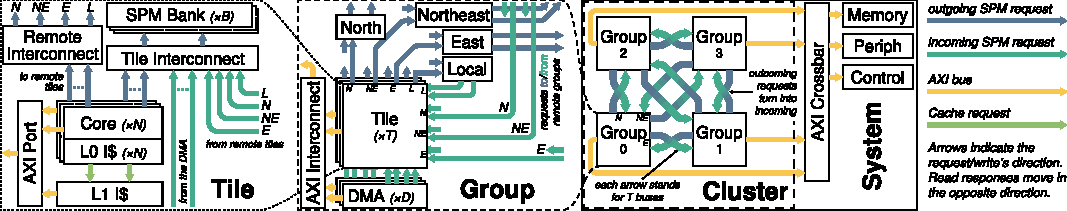
\includegraphics[width=\textwidth]{./fig/mempool.pdf}
	\caption{MemPool's Architecture Hierarchy.}%
	\label{fig:mempool}
\end{figure}

\subsection{Architecture Overview}
\label{subsec:mempool_architecture}

At the heart of MemPool lies the \emph{Snitch} core, which is a simple, in-order, 32-bit RISC-V
core. This core was adapted for this architecture by adding the ability to retire out-of-order load
instructions, which, in addition to its previously existing support for issuing multiple outstanding
loads and stores through scoreboarding, allows MemPool to completely hide the L1 access latency.

MemPool's architecture is hierarchical and comprised of the following building blocks:

\paragraph{Tile} A tile is made up of a number of cores, some shared L1 banks, an L1 instruction
cache shared amongst the tile's cores, as well as a set of remote ports to send/receive requests
to/from other tiles trying to access the global L1 cache. Although any region of the L1 cache is
accessible by any tile, obtaining data from remote tiles is more costly than reading/writing it
directly from/to the local banks. Finally, it also has an \gls{axi} port connected to the system
bus, which allows the tile to access the global L2 cache or system memory.

\paragraph{Group} A group is made up of multiple tiles. Each tile's remote ports are connected with
each other both within the same group as well as with other groups through a series of
interconnects. Each tile's \gls{axi} port is connected to the rest of the system, also supporting
\gls{dma}.

\paragraph{Cluster} Finally, a cluster is made up of multiple groups. Here, an \gls{axi} interface
is used to connect MemPool to the rest of the system (e.g., L2 cache, system memory, etc.).

Another interesting aspect of MemPool's architecture is the \emph{hybrid memory addressing scheme}.
MemPool's shared L1 memory is interleaved at the word level across all banks. This means that
accessing any given sequential region of memory would result in many strided accesses to remote
tiles. This is not an issue for data shared across all cores, however, it is needlessly costly for
local data (e.g., the stack). For this reason, MemPool is able to dedicate \emph{sequential regions}
of memory that are interleaved only within the same tile by re-interpreting the memory address,
which is entirely done in hardware.

\subsection{Programming Model}

MemPool aims to provide a conceptually simple and familiar programming model to ease the development
of parallel applications. It is based on the following principles:

\begin{enumerate}
	\item Shared memory: MemPool provides a shared memory programming model, which means that all
	      cores have access to the full shared memory space.
	\item Independently programmable cores: Each core is individually programmable, which means that
	      each core can execute different code at the same time unlike on GPUs or SIMD architectures.
\end{enumerate}

\section{OpenMP}
\label{sec:openmp}

In her report~\cite{herokmp}, \citeauthor{herokmp} provides a comprehensive overview of OpenMP and
its most commonly used constructs and clauses. In this work, we will implement all of the ones
mentioned in her work, as well as the \emph{teams} construct, described in the following:

The \emph{teams} construct uses the following syntax:

\begin{lstlisting}[language=C, caption={teams construct}, label={lst:teams}]
#pragma omp teams [clause[ [,] clause] ... ] new-line
  structured-block
\end{lstlisting}

with the following clauses:

\begin{lstlisting}[language=C, caption={teams clauses}, label={lst:teams-clauses}]
num_teams(scalar-integer-expression)

thread_limit(scalar-integer-expression)

default(shared | firstprivate | private | none)

private(list)

firstprivate(list)

shared(list)

reduction([default ,] reduction-identifier : list)

allocate([allocator :] list)
\end{lstlisting}

The \emph{teams} construct is used to create a league of teams, where each team is a group of
threads. The number of teams is less then or equal to the value defined by the \emph{num\_teams}
clause, and the maximum number of threads in each team is less than or equal to the value defined by
the \emph{thread\_limit} clause.

The \emph{structured_block} is able to contain other OpenMP constructs such as \emph{parallel},
meaning that this construct essentially allows the creation of independent groups of threads, each
of which could work on different tasks. This is particularly useful in the context of MemPool, as
it allows for the creation of multiple teams, each of which could be assigned to a different tile or
group (or even to different clusters in a multi-cluster system).
